\documentclass[9pt]{article}%
\usepackage[margin=2cm]{geometry}%
\usepackage{subcaption}


\usepackage{listings}
\usepackage{rotating}
\usepackage{xcolor}
\usepackage{graphicx}
\usepackage{enumitem,amssymb,pdfpages}



\definecolor{cmdWhite}{RGB}{255,255,255}
\definecolor{cmdBlack}{RGB}{0,0,0}


\lstdefinestyle{cmdoutput}{
    frame = single,
    belowcaptionskip=1\baselineskip,
    breaklines=true,
    numbers=left,
    xleftmargin=\parindent,
    language=C++,
    showstringspaces=false,
    basicstyle=\footnotesize\ttfamily\color{cmdBlack},
    keywordstyle=\bfseries\color{cmdBlack},
    commentstyle=\itshape\color{cmdBlack},
    identifierstyle=\color{cmdBlack},
    stringstyle=\color{cmdBlack},
    backgroundcolor=\color{cmdWhite},
    rulecolor=\color{cmdBlack},
    rulesepcolor=\color{cmdBlack},
    escapeinside={\%LISTING:}{\^^M},
    xleftmargin=0.5cm,
    xrightmargin=0.5cm,
}




\title{Name Surname Student number}
\author{}
\begin{document}%



\maketitle

\subsection*{compile\textunderscore log.txt}



\noindent\begin{lstlisting}[style=cmdoutput,numbers=none]
Output:
Errors:

Other files:  Checkerboard.cpp Checkerboard.h input.txt main.cpp results.txt run name.aux name.log name.pdf name.tex
\end{lstlisting}
\section*{run\textunderscore log.txt}
Console output goes here

\section*{game\textunderscore results\textunderscore log.txt}
\begin{lstlisting}[style=cmdoutput,numbers=none]
Ratings for init 1:  [2,1,1,1]  avg = 1.25 Functionality: P
Ratings for init 2:  [2,2,2,2]  avg = 2.0 Functionality: A

Ratings max:  [2,2,2,2]  avg = 2.0 Functionality: A

###########################################

INITIALIZATION 1

Board size:              6

Recorded pieces left p1: 4
Actual pieces left p1:   4
Directions of p1:        UP = 13  DOWN = 0

Recorded pieces left p2: 0
Actual pieces left p2:   0
Directions of p2:        UP = 0  DOWN = 11

Totals match:            Yes

Penalties:

Label penalty:           0
Invalid moves made:      13
Compulsory move penalty: 0
Totals match penalty:    0
Win condition penalty:   0
Alternating dir penalty: 0


Functionalty rating:  A

------------------------------------------

INITIALIZATION 2

Board size:              6

Recorded pieces left p1: 4
Actual pieces left p1:   4
Directions of p1:        UP = 13  DOWN = 0

Recorded pieces left p2: 0
Actual pieces left p2:   0
Directions of p2:        UP = 0  DOWN = 11

Totals match:            Yes

Penalties:

Label penalty:           0
Invalid moves made:      1
Compulsory move penalty: 0
Totals match penalty:    0
Win condition penalty:   0
Alternating dir penalty: 0


Functionalty rating:  A

###########################################

###########################################

INITIALIZATION 1

Board size:              8

Recorded pieces left p1: 3
Actual pieces left p1:   3
Directions of p1:        UP = 32  DOWN = 0

Recorded pieces left p2: 2
Actual pieces left p2:   2
Directions of p2:        UP = 0  DOWN = 36

Totals match:            Yes

Penalties:

Label penalty:           0
Invalid moves made:      27
Compulsory move penalty: 8
Totals match penalty:    0
Win condition penalty:   1
Alternating dir penalty: 0


Functionalty rating:  P

------------------------------------------

INITIALIZATION 2

Board size:              8

Recorded pieces left p1: 3
Actual pieces left p1:   3
Directions of p1:        UP = 32  DOWN = 0

Recorded pieces left p2: 2
Actual pieces left p2:   2
Directions of p2:        UP = 0  DOWN = 36

Totals match:            Yes

Penalties:

Label penalty:           0
Invalid moves made:      3
Compulsory move penalty: 8
Totals match penalty:    0
Win condition penalty:   1
Alternating dir penalty: 0


Functionalty rating:  A

###########################################

###########################################

INITIALIZATION 1

Board size:              10

Recorded pieces left p1: 10
Actual pieces left p1:   10
Directions of p1:        UP = 53  DOWN = 0

Recorded pieces left p2: 1
Actual pieces left p2:   1
Directions of p2:        UP = 0  DOWN = 51

Totals match:            Yes

Penalties:

Label penalty:           0
Invalid moves made:      41
Compulsory move penalty: 19
Totals match penalty:    0
Win condition penalty:   1
Alternating dir penalty: 0


Functionalty rating:  P

------------------------------------------

INITIALIZATION 2

Board size:              10

Recorded pieces left p1: 10
Actual pieces left p1:   10
Directions of p1:        UP = 53  DOWN = 0

Recorded pieces left p2: 1
Actual pieces left p2:   1
Directions of p2:        UP = 0  DOWN = 51

Totals match:            Yes

Penalties:

Label penalty:           0
Invalid moves made:      1
Compulsory move penalty: 6
Totals match penalty:    0
Win condition penalty:   1
Alternating dir penalty: 0


Functionalty rating:  A

###########################################

###########################################

INITIALIZATION 1

Board size:              12

Recorded pieces left p1: 12
Actual pieces left p1:   12
Directions of p1:        UP = 70  DOWN = 0

Recorded pieces left p2: 5
Actual pieces left p2:   5
Directions of p2:        UP = 0  DOWN = 68

Totals match:            Yes

Penalties:

Label penalty:           0
Invalid moves made:      56
Compulsory move penalty: 12
Totals match penalty:    0
Win condition penalty:   0
Alternating dir penalty: 0


Functionalty rating:  P

------------------------------------------

INITIALIZATION 2

Board size:              12

Recorded pieces left p1: 17
Actual pieces left p1:   17
Directions of p1:        UP = 70  DOWN = 0

Recorded pieces left p2: 0
Actual pieces left p2:   0
Directions of p2:        UP = 0  DOWN = 68

Totals match:            Yes

Penalties:

Label penalty:           0
Invalid moves made:      1
Compulsory move penalty: 15
Totals match penalty:    0
Win condition penalty:   0
Alternating dir penalty: 0


Functionalty rating:  A

###########################################

results.txt contents 

6
p1 13-11
p2 4-7
p1 11x4(7)
p2 6-8
p1 17-13
p2 3-6
p1 13-11
p2 8x13(11)
p1 16x11(13)
p2 5-7
p1 15-12
p2 6-8
p1 11x6(8)
p2 2x9(6)
p1 18-15
p2 1-5
p1 4-1
p2 5-8
p1 12x5(8)
p2 9-12
p1 15x8(12)
p2 7-11
p1 14x7(11)
p1 14x7(11)
tp1 4
tp2 0
wp2

8
p1 23-18
p2 10-15
p1 22-17
p2 15x22(18)
p1 25x18(22)
p2 7-10
p1 18-14
p2 3-7
p1 17-13
p2 12-16
p1 29-25
p2 8-12
p1 27-23
p2 16-20
p1 23-19
p2 10x17(14)
p1 21x14(17)
p2 12-16
p1 19x12(16)
p2 9x18(14)
p1 13-9
p2 6x13(9)
p1 26-23
p2 7-10
p1 23x14(18)
p2 10x17(14)
p1 31-26
p2 20x27(24)
p1 32x23(27)
p2 1-6
p1 23-19
p2 5-9
p1 26-22
p2 2-7
p1 19-15
p2 17x26(22)
p1 15x8(11)
p2 4x11(8)
p1 30x23(26)
p2 9-14
p1 25-21
p2 6-9
p1 28-24
p2 13-17
p1 24-19
p2 14-18
p1 23x14(18)
p2 11-16
p1 14x5(9)
p2 16x23(19)
p1 21x14(17)
p2 7-11
p1 14-10
p2 11-16
p1 10-7
p2 23-27
p1 7-2
p2 16-19
p1 5-1
p2 19-24
p1 12-8
p2 27-32
p1 8-4
p2 24-27
p2 24-27
p2 27-31
p2 27-31
p2 27-31
tp1 3
tp2 2
wp2

10
p1 33-29
p2 17-21
p1 35-30
p2 12-17
p1 32-28
p2 20-25
p1 28-23
p2 18-22
p1 38-32
p2 19x28(23)
p1 32x23(28)
p2 13-18
p1 23x12(18)
p2 7x18(12)
p1 39-33
p2 8-12
p1 30-24
p2 1-7
p1 40-35
p2 22-28
p1 33x22(28)
p2 14-20
p1 22x13(18)
p2 9x18(13)
p1 37-32
p2 18-22
p1 32-28
p2 22x33(28)
p1 42-37
p2 33-39
p1 44x33(39)
p2 25-30
p1 34x25(30)
p2 17-22
p1 25x14(20)
p2 10x19(14)
p1 24x13(19)
p2 2-8
p1 13x2(8)
p2 3-8
p1 50-44
p2 12-17
p1 29-23
p2 5-10
p1 44-40
p2 21-27
p1 33-29
p2 7-12
p1 23-19
p2 22-28
p1 31x22(27)
p2 10-14
p1 19x10(14)
p2 4-9
p1 37-32
p2 28x37(32)
p1 41x32(37)
p2 16-21
p1 49-44
p2 12-18
p1 22x13(18)
p2 8x19(13)
p1 40-34
p2 9-14
p1 10-5
p2 14-20
p1 45-40
p2 20-24
p1 29x20(24)
p2 17-22
p1 43-39
p2 15x24(20)
p1 48-42
p2 24-29
p1 34x23(29)
p2 19x28(23)
p1 32x23(28)
p2 22-27
p1 39-33
p2 11-16
p1 36-31
p2 6-11
p1 31x22(27)
p2 21-26
p1 40-34
p2 11-17
p1 22x11(17)
p2 26-31
p1 42-38
p2 16-21
p1 44-39
p2 31-37
p1 23-18
p2 21-26
p1 47-42
p2 37x48(42)
p1 18-12
p2 26-31
p1 11-6
p2 31-37
p1 12-8
p2 37-41
p1 46x37(41)
p1 46x37(41)
tp1 10
tp2 1
wp2

12
p1 47-40
p2 26-33
p1 48-42
\end{lstlisting}


\begin{figure}[ht!]
\vfill\eject
\begin{subfigure}{0.4\textwidth}
   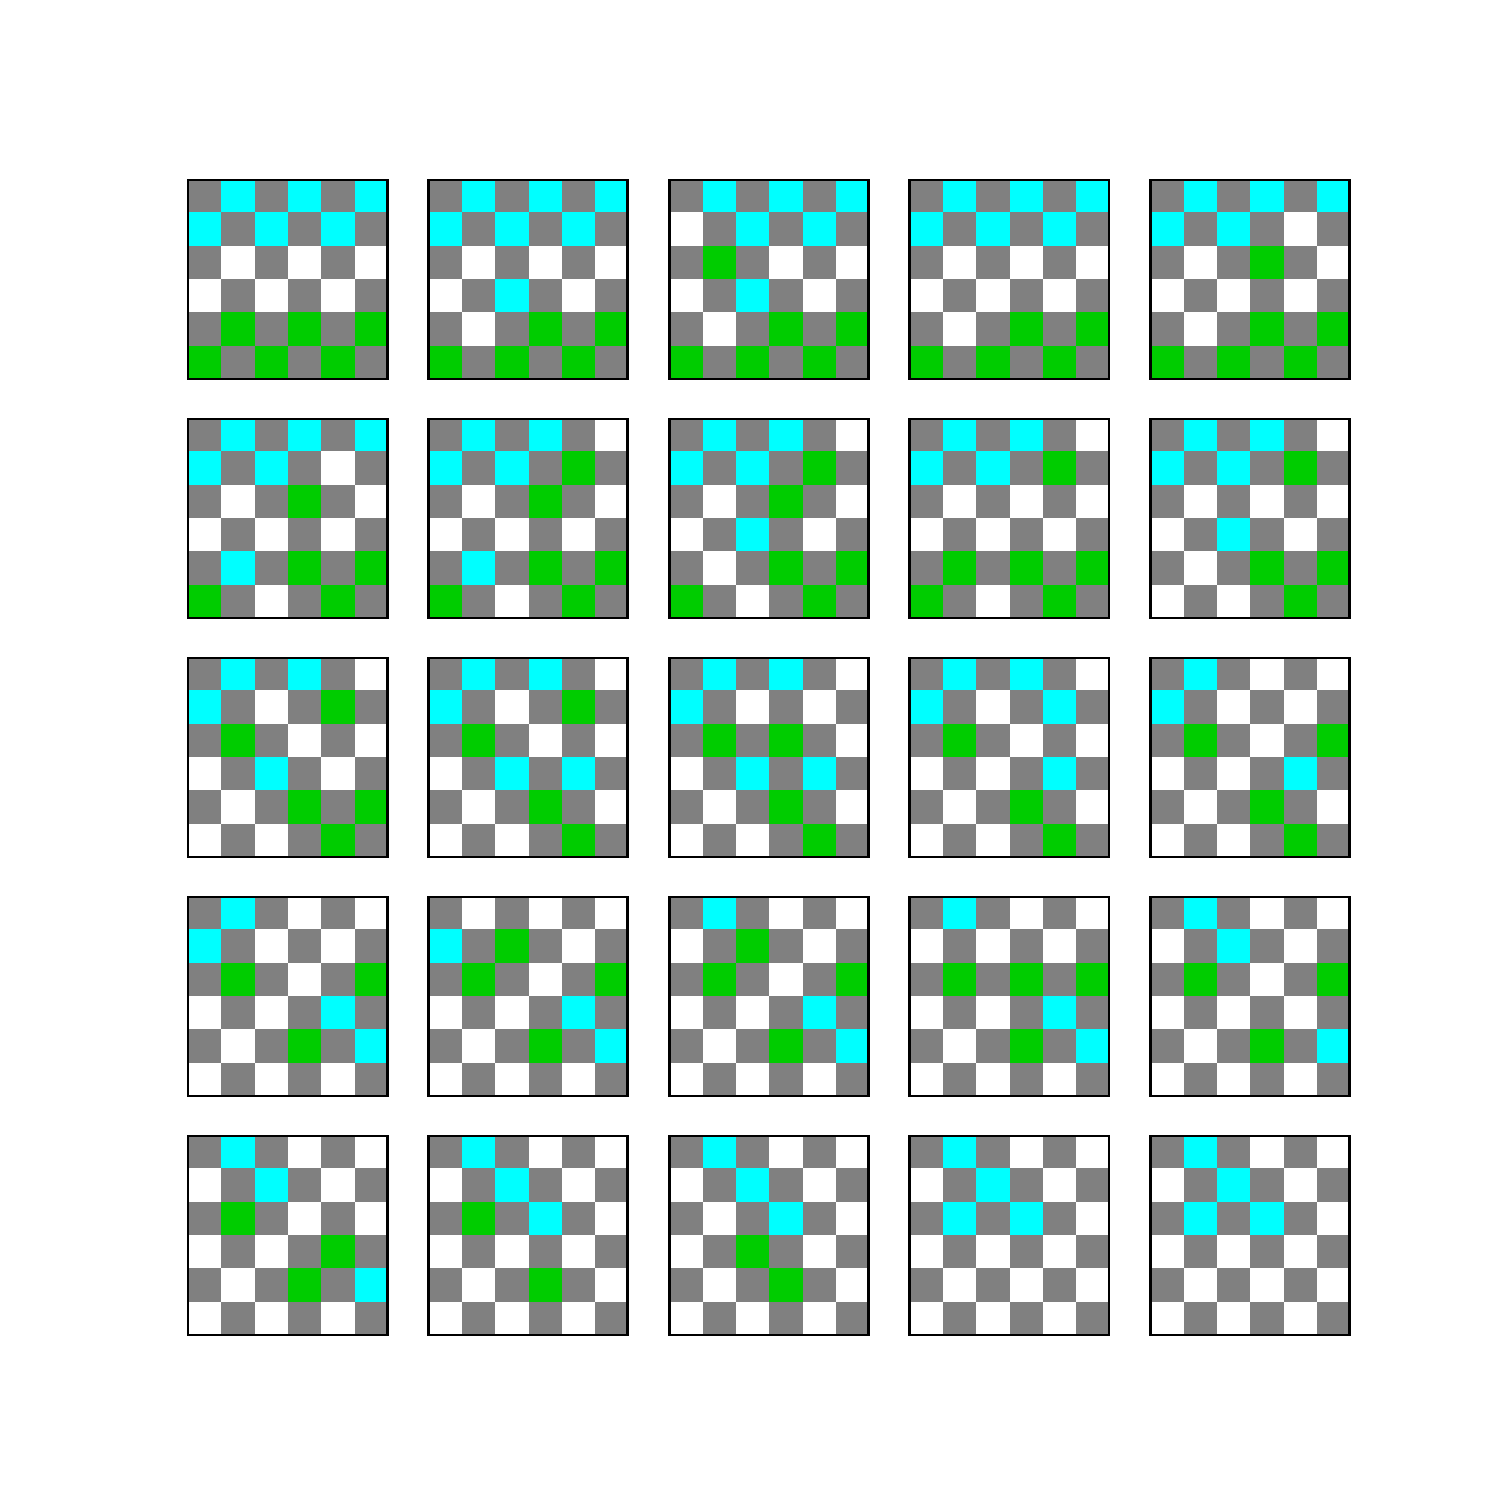
\includegraphics[width=\textwidth]{games_0_init1.pdf}
   \caption{games-0-init1.pdf} 
   \end{subfigure}~
   \begin{subfigure}{0.4\textwidth}
   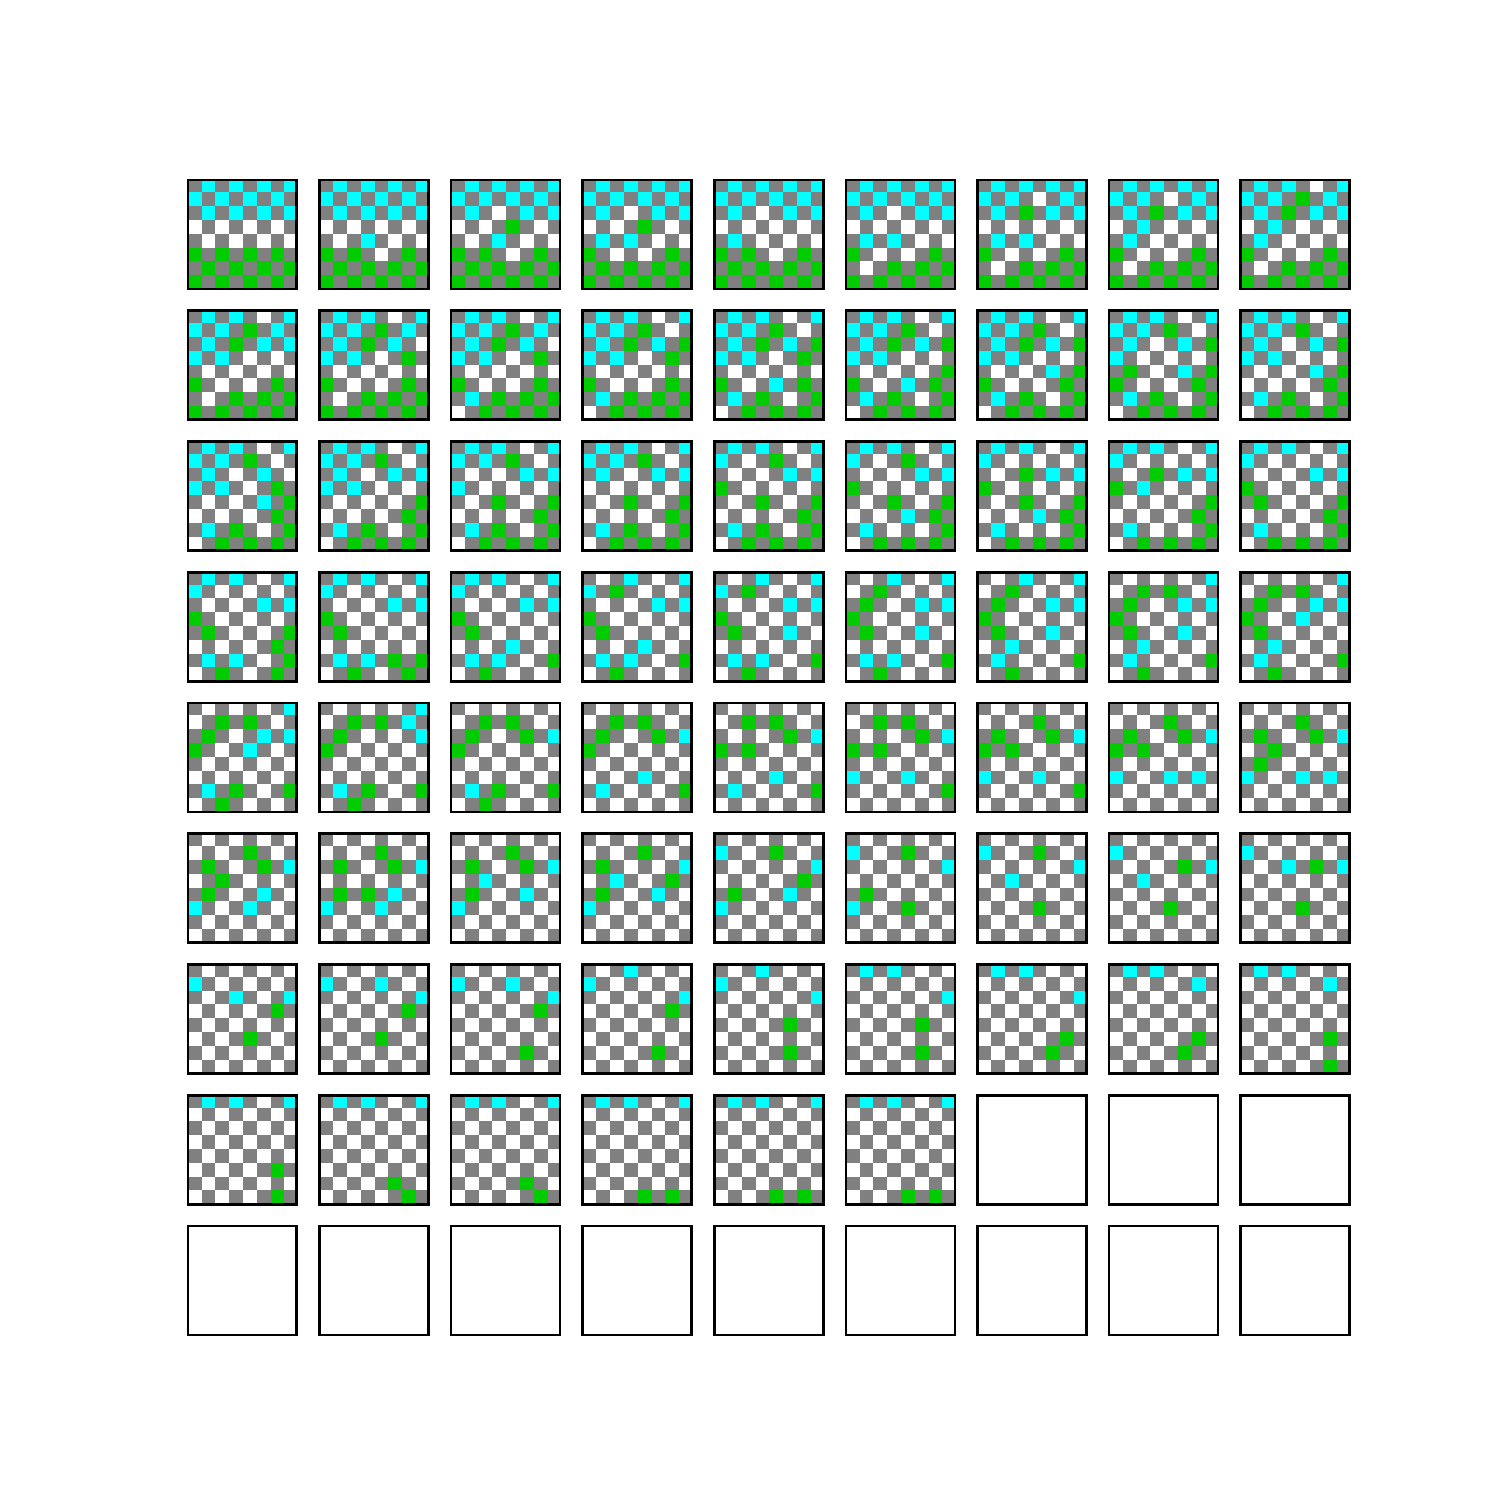
\includegraphics[width=\textwidth]{games_1_init1.pdf}
   \caption{games-1-init1.pdf}
   \end{subfigure}
\vfill\eject
\end{figure}


\section*{source code}

\begin{lstlisting}[caption=Checkerboard.cpp,style=cmdoutput]
#include "Checkerboard.h"

//<num>

#include <iostream>
#include <vector>
#include <ctime> //time()
#include <cstdlib> //rand()
#include <string>

using namespace std;

/*Checkerboard::Checkerboard()
{
    //ctor
}*/

void Checkerboard::printBoard(vector <vector<char >> &v) //Allows me to see what is happening on the board in real-time even though it  raises the complexity of the code
{
    for(int i = 1; i <= boardsize; i++)
          {

//Students code
     string s = "";
    s = "tp2 " + to_string(Xcount);
    return s;
}

\end{lstlisting}

\begin{lstlisting}[caption=Checkerboard.h,style=cmdoutput]
#ifndef CHECKERBOARD_H
#define CHECKERBOARD_H


#include <iostream>
#include <vector>
#include <ctime> //time()
#include <cstdlib> //rand()
#include <string>
//students code
#endif // CHECKERBOARD_H
\end{lstlisting}

\begin{lstlisting}[caption=main.cpp,style=cmdoutput]
#include "Checkerboard.h"

#include <iostream>
#include <fstream>
#include <vector>
#include <ctime> //time()
#include <cstdlib> //rand()
#include <string>

using namespace std;

int main()
{
//students code
}
\end{lstlisting}

\end{document}